
% \begin{figure}[tb]
% \begin{center}
%     \centering
%   \caption{Posterior predictive loss (Left) and energy score (right) for various models on simulated data.  Gen indicates baseline.\label{fig:simpples}}
%   \begin{subfigure}[b]{0.48\textwidth}
%     \centering
%     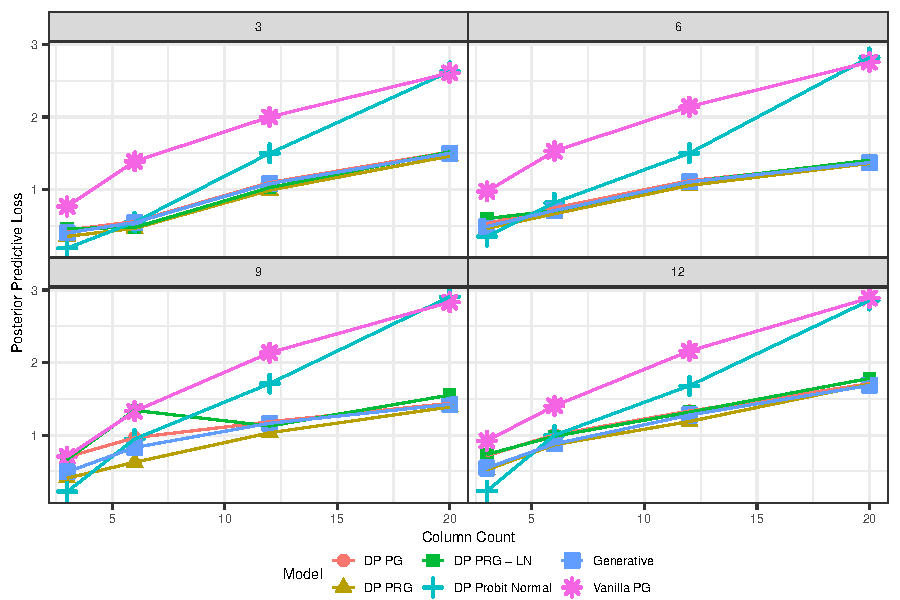
\includegraphics[height=2in, width=\textwidth]{./images/simulation_ppl}
%   \end{subfigure}
%   %
%   \begin{subfigure}[b]{0.48\textwidth}
%     \centering
%     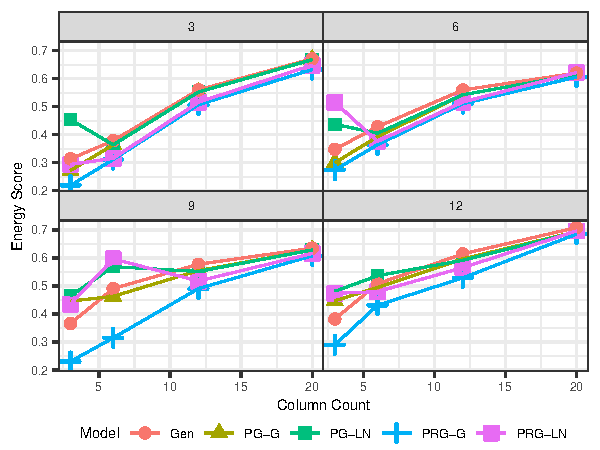
\includegraphics[height=2in, width=\textwidth]{./images/simulation_es}
%   \end{subfigure}
% \end{center}
% \end{figure}

\begin{figure}[htb]
    \centering
    \caption{Energy score (top row) and Posterior Predictive Loss (bottom row) for various models on simulated data with ascending count of mixture components (indicated by plot heading) and number of dimensions (indicated by horizontal axis).  Gen indicates baseline.\label{fig:simpples}}
    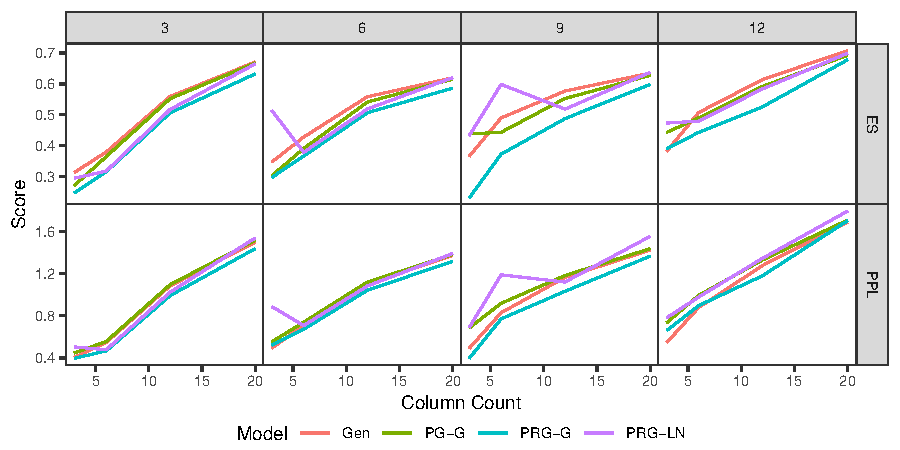
\includegraphics[height=3in, width = \textwidth]{./images/simulation_score}
\end{figure}


\section{Data illustrations\label{sec:results}}

\subsection{Simulations\label{subsec:simulated}}

To evaluate our proposed approach for angular measure estimation 
we consider simulated datasets on $\mathbb{S}_{\infty}^{d-1}$, for 
$d$ ranging between 3 and 20. We generated each dataset from a mixture of projected Gammas, with the number of mixture components
  ranging between 3 and 12.  The generation procedure is detailed in Algorithm~\ref{algo:simulated}.
  \begin{algorithm}[ht]
    \footnotesize
    \caption{Simulated Angular Dataset Generation Routine\label{algo:simulated}}
    \For{$n_{\text{mix}}$ in $[3, 6, 9, 12]$}{
      Generate $n_{\text{mix}} \times 20$ shape Parameters $\alpha$\\
      Generate $n_{\text{mix}} \times 20$ Rate Parameters $\beta$\\
      Generate $500$ Mixture Component Identifiers $\delta$\\
      \For{$i$ in $1,\ldots,500$}{
        Generate ${\bf X}_i \sim \prod_{\ell = 1}^d\text{Ga}\left(X_{il}\mid\alpha_{\delta_i,l},\beta_{\delta_i, l}\right)$
        }
      \For{$n_{\text{col}}$ in $[3,6,12,20]$}{
        Project columns 1 to $n_{\text{col}}$ of ${\bf X}$ onto 
        $\mathcal{S}_{\infty}^{n_{\text{col}} - 1}$ and save.
        }
    }
  \end{algorithm}
Each one of the shape parameters $\alpha$ were generated 
$\alpha = \alpha_0 + \alpha_1$ where
  $\alpha_0 \sim \text{Unif}(\alpha_0\mid 0,4)$, $\alpha_1\sim \text{Gamma}(\alpha_1\mid 1,1)$.
The scale parameters $\beta$ were obtained as $\beta\sim\text{Unif}(\beta\mid 0.25, 2.5)$.

% \begin{figure}[ht]
%   \caption{Simulation Energy Score versus Column Count, by Mixture Component Count. Lower is better.\label{fig:simes}}
%   \centering
%   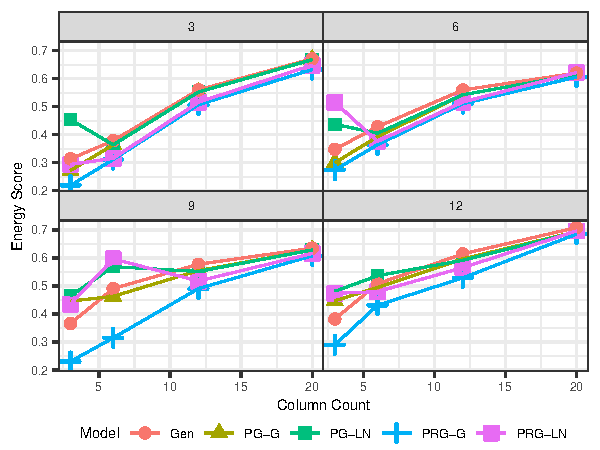
\includegraphics[width=0.8\textwidth]{./images/simulation_es}
% \end{figure}

Figure~\ref{fig:simpples}, shows two sets of panels that illustrate the comparison
between four different models used to fit the simulated data. We produced 16 
different data sets, one for each of four different numbers of mixture components 
and four different dimensions. We considered three different models: DP mixtures 
of projected gamma; Projected restricted gamma; and projected restricted gamma 
with a multivariate log-normal prior. We calculated $S^\infty_{\text{PPL}}$ and 
$S_{\text{ES}}$ using predictive samples from each of fitted models. To provide 
a comparative baseline, we calculated the scores using samples generated 
directly using the same model and parameters that produced the simulated 
observations. The results are denoted as \emph{Gen} in the figure. 
We observe that the projected
  restricted Gamma model dominates in most situations, but the difference between projected restricted
  Gamma and the other gamma-based models tends to shrink as the number of dimensions increases.
  Alternatively, that difference appears to grow as the number of mixture components increases. 
  The results from both scoring criteria are comparable.

% We frequently see all of the gamma-based mixture models accomplish a lower energy score
%     than the generative distribution.  As \cite{nunez2019} noted, the projected Gamma model
%     is flexible and can generate multimodal distributions from a single mixture component.
%     When we allow a mixture model, we allow the possibility to break those modes into 
%     different mixture components.  This will tend to result in a better energy score, as 
%     posterior predictive replicates for a given observation in a local model will tend to 
%     be concentrated in that local mode rather than being spread between multiple modes.  
%     As for the dominance of projected restricted Gamma, By specifying $\beta_{\ell} := 1$ 
%     for all $l$, if there were multi-modal mixture components, we are in effect breaking 
%     the mixture components into separate modes. As for whether this represents 
%     \emph{overfitting}, If we had reason to believe that the generative distribution for
%     real data followed this form, then such a case could be made.  However, we are using 
%     projected Gamma as a parametric stand-in for an unknown distribution. In this sense, 
%     the argument for overfitting is less clear.
%     {\bf This paragraph is not very clear. Please make an effort to tell the story more clearly.}

\subsection{Integrated Vapor Transport\label{subsec:ivt}}
The \emph{integrated vapor transport} (IVT) is a two component vector 
that tracks the flow of the total water volume in a column of air 
over a given area \citep{ralph2017}.  IVT is increasingly used in the study of atmospheric rivers because of its direct 
relationship with orographically induced precipitation
\citep{neiman2009water}. Atmospheric rivers (AR) are elongated areas of high 
local concentration of water vapor in the atmosphere that transport water
from the tropics around the world. AR can cause extreme 
precipitation,  something that is usually associated with very large values
of the IVT magnitude over a whole geographical area. In spite of this, AR
are fundamental for the water supply of areas like California. Thus the
importance of understanding the extreme behavior of IVT, including 
extreme tail dependence. We consider datasets that correspond to IVT
estimated at two different spatial resolutions. The coarse resolution dataset
is obtained from the European Centre for Medium-Range Weather Forecasts
(ECMWF) Interim reanalysis (ERA-Interim) \citep{berrisford2011atmospheric,dee2011era}. 
The high resolution dataset corresponds to the latest ECMWF 
observational product, ERA5  \citep{hersbach2020era5}. 

\begin{figure}[tb]
    \begin{center}
    \caption{Grid cell locations for ERA-Interim (left) and ERA5 (right).\label{fig:gridlocs}}
    \begin{subfigure}[b]{0.48\textwidth}
        \centering 
        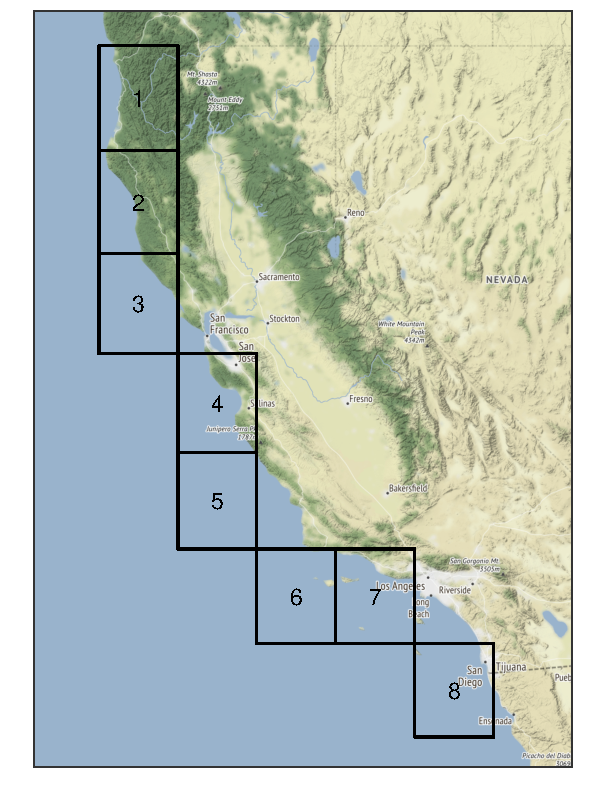
\includegraphics[height=2.5in]{./images/erai_grid}
    \end{subfigure}
    %
    \begin{subfigure}[b]{0.48\textwidth}
        \centering
        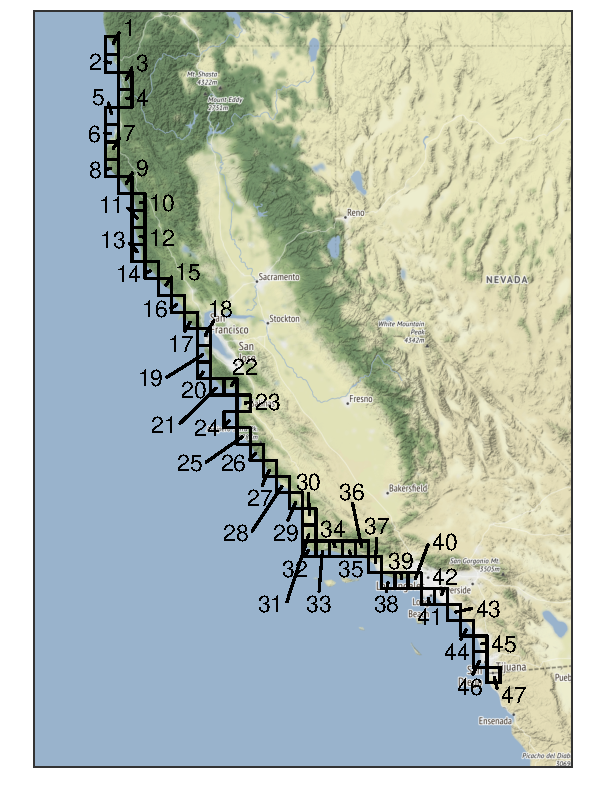
\includegraphics[height=2.5in]{./images/era5_grid}
    \end{subfigure}
    \end{center}
\end{figure}

Our data corresponds to daily average values for the IVT magnitude
along the coast of California.  The ERA-Interim data used covers the time period 
1979 through 2014 (37 years) omitting leap days, and eight grid cells that correspond to the coast of California.  The ERA5 data
covers the time period 1979 through 2019 (42 years) with the same restriction, and 
47 grid cells for the coast of California.  This gives us the opportunity to illustrate the performance of our method 
in multivariate settings of very different dimensions. Figure~\ref{fig:gridlocs} provides a visual representation of the area these grid cells represent.

\begin{algorithm}[htb]
    \footnotesize
   \caption{Data preprocessing to isolate and transform data exhibiting extreme behavior.  $r_i$
   represents the radial component, and $\bm{v}_i$ the angular component.  The declustering
   portion is relevant for data correlated in time.\label{algo:processing}}
  \KwResult{$\bm{ r},\bm{v} : r_i \sim \text{Pareto}(1)$, $\bm{ v}_i \in {\mathbb S}_{\infty}^{d-1}$}
  \For{$\ell = 1,\ldots,d$}{
    Set $b_{t,\ell} = \hat{F}_{\ell}^{-1}\left(1 - \frac{1}{t}\right)$.\\
    With $\bm{ x}_{\ell} > b_{t,\ell}$, fit $a_{\ell}$, $\xi_{\ell}$ via MLE according to generalized Pareto likelihood.\\
    }
  \For{$i = 1,\ldots,n$}{
    Define $z_{i,\ell} = \left(1 + \xi_{\ell}\frac{x_{i,\ell} - b_{t,\ell}}{a_{\ell}}\right)_{+}^{1/\xi_{\ell}}$; $\;\;\;$ then $r_i = \pnorm{\bm{ z}_i}{\infty}$, $\;\;\bm{ v}_i = \frac{\bm{ z}_i}{\pnorm{\bm{ z}_i}{\infty}}$\\
    }
  Subset $\bm{ r},\bm{ v}$ such that $r_i \geq 1$\\
  \If{declustering}{
    \For{$i = 1,\ldots,n$}{
      If $r_i \geq 1$ and $r_{i-1} \geq 1$, drop the lesser (and associated $v_i$) from data set.\\
    }
  }
\end{algorithm}

\begin{figure}[ht]%{l}{0.45\textwidth}
    \centering
    \caption{Pairwise plots from ERA-Interim data after transformation and projection to ${\mathbb S}_{\infty}^{7}$.  Down the diagonal are marginal kernel densities, with two-dimensional histograms on the off-diagonal.  In those plots, red indicates a higher density.  All data is between 0 and 1.\label{fig:erai_data}}
    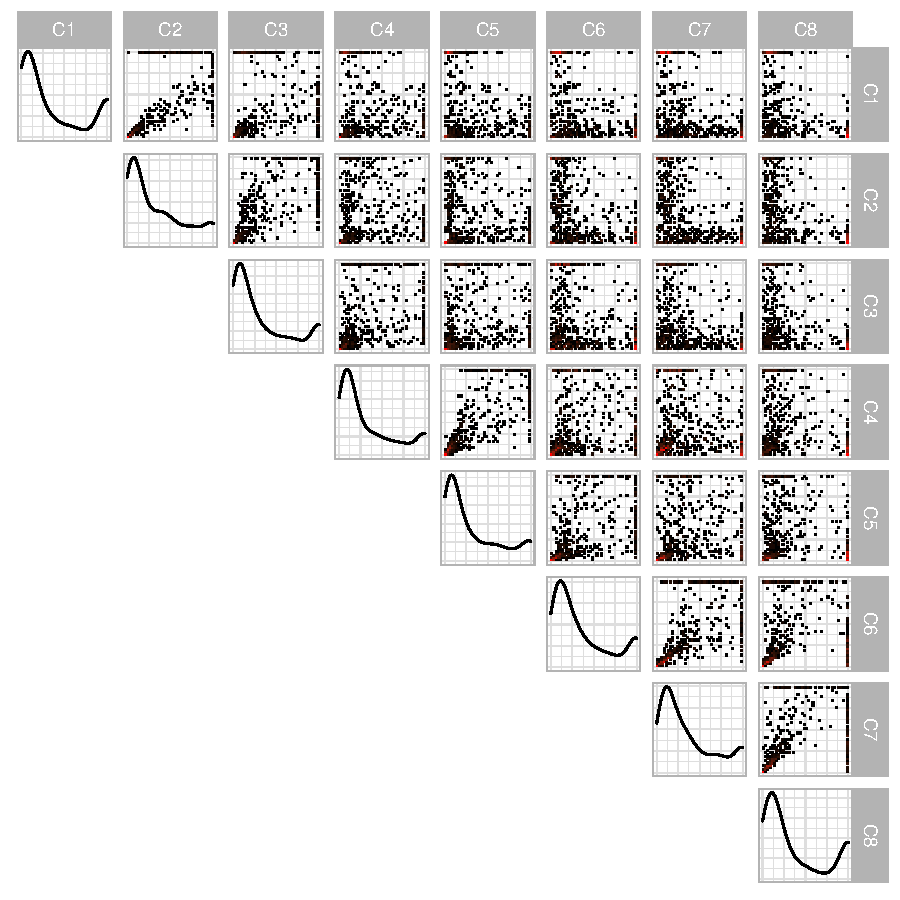
\includegraphics[width=.7\linewidth]{./images/data_transformed}
\end{figure}

Fitting our models to the IVT data requires some pre-processing. First, we subset the data to the rainy
  season, which in California runs roughly from November to March.  Following the approach described 
  in Section \ref{sec:methodology} we estimate the shape and scale parameters of a univariate GP, in each
  dimension, using maximum likelihood. We set the threshold in each dimensions $\ell$ as  
  $b_{t,\ell} = \hat{F}_{\ell}^{-1}(1 - t^{-1})$, where $\hat{F}$ is the empirical CDF and $t=20$, 
  that corresponds to the $95$ percentile. We then use the transformation in Equation
  \eqref{eqn:standardization} to standardize the observations.  Dividing each standardized observation
  by its $\mathcal{L}_{\infty}$ norm, we obtain a projection onto $\mathcal{S}_{\infty}^{d-1}$. As 
  the data correspond to a daily time series, the observations are temporally correlated.  For each
  group of consecutive standardized vectors $z_i$ such  that  $\inorm{z_i} > 1$, we retain only the
  vector with the largest $\mathcal{L}_{\infty}$ norm.  The complete procedure is outlined in
  Algorithm~\ref{algo:processing}.  
  
After subsetting the ERA-Interim data to the rainy season we 
  have $5587$ observations. After the processing and declustering described in
  Algorithm~\ref{algo:processing}, this number reduces to $511$ observations. A pairwise plot 
  of the transformed data after processing and declustering is presented in 
  Figure~\ref{fig:erai_data}.  From this, we note that the marginal densities display strong
  similarities, with a large spike near 0 and a small spike near 1. A value of 1 in a particular 
  axis indicates that the standardized threshold exceedance was largest in that dimension.  
  The off-diagonal plots correspond to pairwise density plots.  We observe that some site pairs, such 
  as $(1,2)$, $(7,8)$, and especially $(4,5)$ have the bulk of their data concentrated in a 
  small arc along the $45^{\circ}$, while other site combinations such as $(3,6)$, $(2,7)$, or
  $(1,8)$ the data is split, favoring one side or the other of the $45^{\circ}$ line. For the 
  ERA5 data, after subsetting we have $6342$ observations, which reduces to $532$ observations 
  after processing and declustering. We fit the PG--G, PRG--G, PG--LN, and PRG--LN models to 
  both datasets.
%  {\bf At this point it would be nice to include a figure with a plot of the data after all the pre-processing. You show a couple of panels for the ERA-Iterim and a couple of the ERA5.}
%  \makenote{Do you mean marginal histograms, or, like, a couple selected ternary scatter-plots?}

\begin{table}[htb]
  \centering
  \caption{Model comparison metrics: Posterior~Predictive~Loss~($S_{\text{PPL}}$) and 
    Energy~Score~($S_{\text{ES}}$) criteria from fitted models against the IVT data.  
    Lower is better. \label{tab:dev}}
  
\begin{tabular}{ccccc}
\toprule
\multicolumn{1}{c}{ } & \multicolumn{2}{c}{dim = 8} & \multicolumn{2}{c}{dim = 47} \\
\cmidrule(l{3pt}r{3pt}){2-3} \cmidrule(l{3pt}r{3pt}){4-5}
Model & PPL & ES & PPL & ES\\
\midrule
PRG & 0.195 & 0.170 & 1.623 & 0.675\\
PRG-LN & 0.232 & 0.192 & 1.400 & 0.582\\
PG & 0.787 & 0.418 & 5.040 & 1.374\\
\bottomrule
\end{tabular}
\end{table}

Table~\ref{tab:dev} shows the values of the estimated posterior predictive loss and energy scores for the different models considered. We observe that, as in the case of the simulation study shown in Figures~\ref{fig:simpples}, the preferred model is the projected restricted 
  gamma models.  Penalization for the unrestricted gamma model is 
  stronger for the real data than for the simulated data. We also observe that
  the restricted gamma model with the log-normal prior performs significantly better 
  than the restricted gamma model with the gamma prior on the higher dimensional data. This is the opposite of the result obtained in the simulation example.

\begin{figure}[ht]
    \centering
    \caption{Pairwise extremal dependence coefficients for IVT data using the PRG--G model.\label{fig:chi_ij}}
    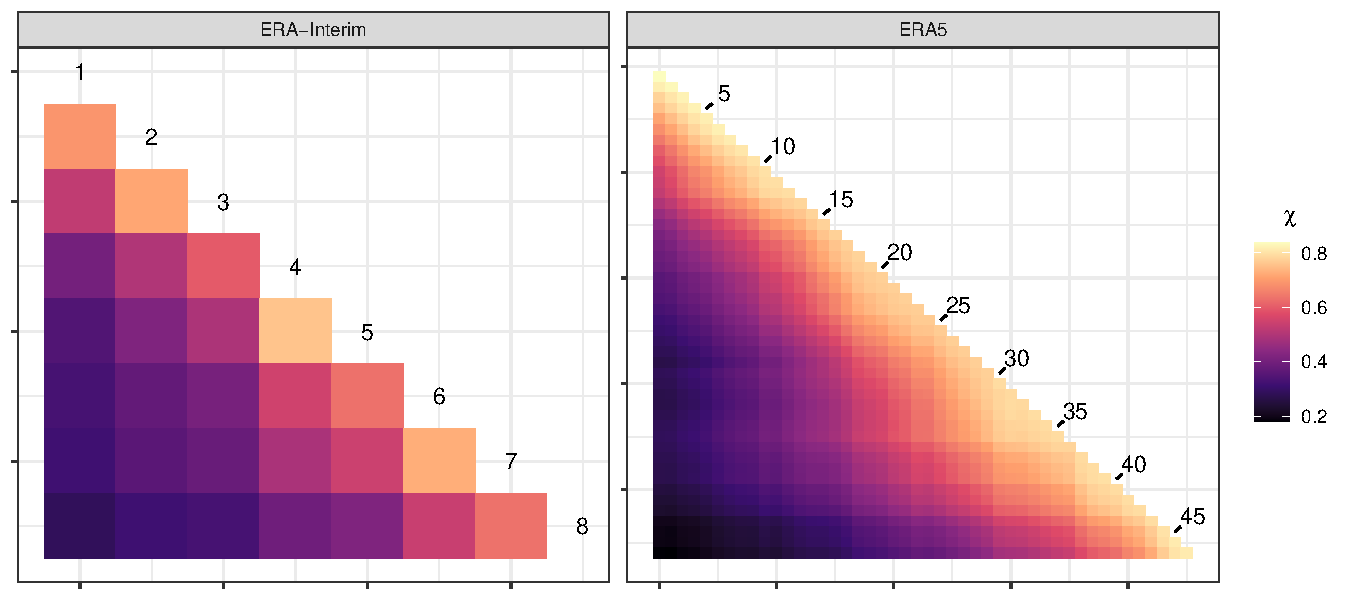
\includegraphics[width=0.9\textwidth]{./images/chi_ij_c}
\end{figure}

We consider an exploration of the pairwise extremal dependence using Monte Carlo estimates of the 
  coefficients in  Equation~\ref{eqn:chi_ij}. For this we use samples obtained from the PRG--G model.
  Figure~\ref{fig:chi_ij} provides a graphical analysis of the results. 
  The coefficients achieve values between $0.286$ and $0.759$ for the ERA-Interim data and 
  between $0.181$ and $0.840$ for the ERA5 data.  The greater range in dependence scores observed 
  with the ERA5 data versus ERA-Interim speaks to the greater granularity of the ERA5 data--distance between locations is a strong contributor to the strength of the 
  pairwise asymptotic dependence. The highest coefficients are $0.759$ for 
  locations 4 and 5 in the ERA-Interim data and
  $0.840$ for locations 1 and 2 in the ERA5 data.  Clearly, pairwise asymptotic
  dependence coefficients tell a limited story, as a particular dependence may include
  more than two locations.   We can, however, glean some information from the patterns that
  emerge in two dimensions.  For the ERA-Interim data, we observe a possible cluster 
  between cells 5-8, indicating a strong dependence among these cells.  Analogously, for
  the ERA5 data, we observe three possible groups of locations.

\begin{figure}[htb]
    \centering
    \caption{Conditional survival curves for selected locations, using ERA-Interim, and PRG-G model,  conditioning on all other dimensions at greater than 90th percentile (fitted)\label{fig:condsurv1d}. The left panel uses original units. Right panel uses standardized units.}
    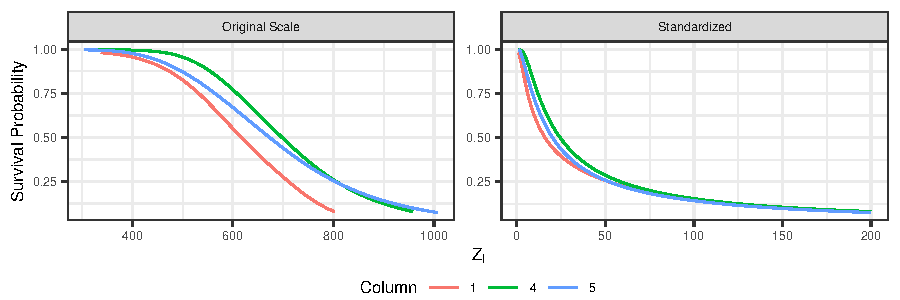
\includegraphics[width=\linewidth]{./images/condsurv_1d}
\end{figure}

\begin{figure}[htb]
    \centering
    \caption{Pairwise conditional survival curves for selected locations, using ERA-Interim, and PRG-G model, conditioning on all other dimensions at greater than 90th percentile (fitted).\label{fig:condsurv2d}}
    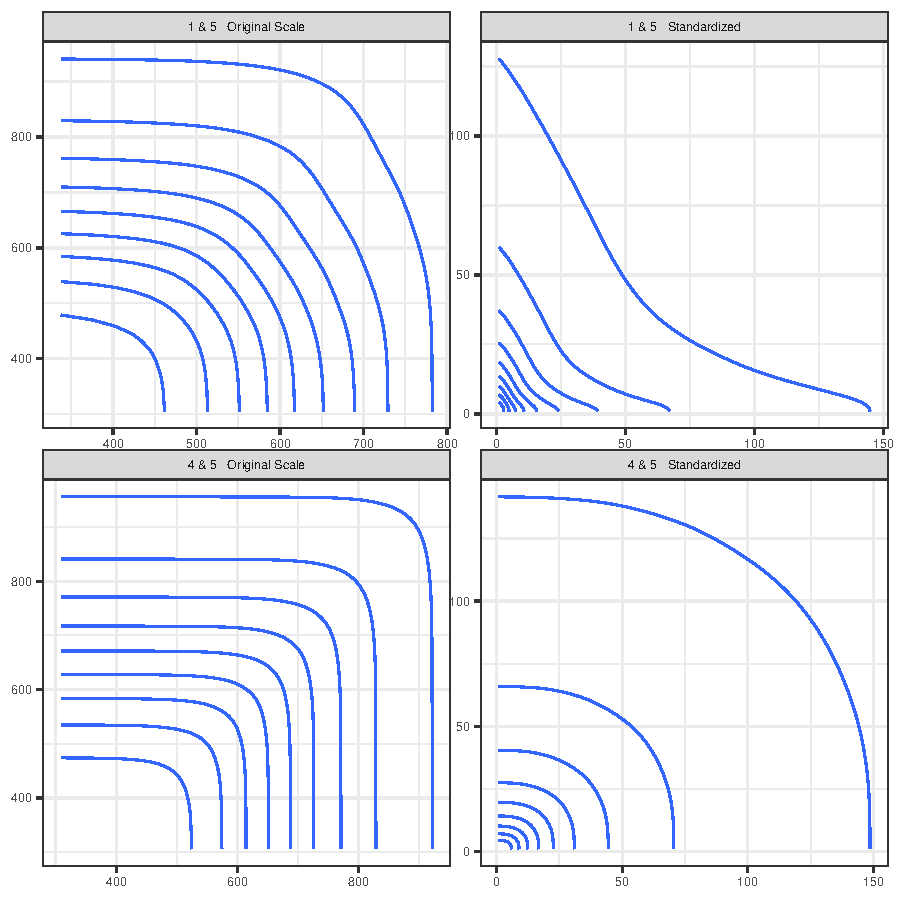
\includegraphics[height=4in, width=4in]{./images/condsurv_2d}
\end{figure}

Figure~\ref{fig:condsurv1d} shows, for the ERA-Interim data under the PRG--G model,  
    the conditional survival curve defined in Equation~\ref{eqn:condsurv}, for one dimension, 
    conditioned on all other dimensions being greater than their (fitted) $90$th percentile. 
    Figure~\ref{fig:condsurv2d} presents the bi-variate conditional survival function,
    conditioning on all other dimensions.  These results illustrate quantitatively how extremal dependence
    affects the shape of the conditional survival curves.  The two top panels represent the joint survival function 
    between grid locations 4 and 5, which are shown in Figure~\ref{fig:chi_ij} to exhibit strong
    extremal dependence.  We observe that the joint survival surface 
    is strongly convex.  The bottom panels represent the joint survival surface between grid locations 1 and 5, 
    which exhibited low extremal dependence.  In this case the shape of the contours tend to be concave, quite different from the shapes observed in the top panels.

Using our proposed scoring criteria, we explored the effect of the choice of $p$ on the final results. Using the simulated data, generated
    from a mixture of projected Gammas, we were unable to observe sizeable differences in the scores for $p$ 
    ranging between 1 and 15.   However, 
    for the IVT data, we observed a drop in the energy score associated 
    with higher $p$, with diminishing effect as $p$ increased.  
    We observed no significant differences in the performance
    of the model that uses $p=10$, which corresponds to the analysis 
    presented, relative to the one that uses $p=15$.
% EOF
